\section{Forces}

% Concept of Force

\subsection{Making a Spring Balance} % Move to Force, Chapter 4

\begin{center}
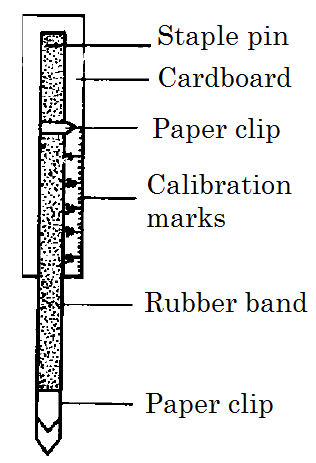
\includegraphics[width=6cm]{./img/source/spring-balance.png}
\end{center}

\begin{description*}
%\item[Subtopic:]{Concept of Force}
%\item[Shika Rating:]{4}
\item[Materials:]{Cardboard, strong rubber band, staple pin, 2 paper clips, \nameref{sec:masses}*}
\item[Setup:]{Take a strip of cardboard or wood and fix a strong rubber band to it using a staple pin. (The stronger the rubber band, the larger the force you can measure.) Attach one paper clip as a pointer as shown in the figure. Then fix another as a hook at the bottom end of the rubber band.}
\item[Procedure:]{Calibrate the balance in \emph{Newtons} using either a standard set of \nameref{sec:masses} or another spring balance. A mass of 10 g has a weight of 0.1 N; a mass of 100 g has a weight of 1 N, etc. Draw marks accordingly on the scale of the balance.}
\item[Hazards:]{Never apply such a large force that the pointer does not return to the zero mark when the force ceases.}
%\item[Questions:]{}
%\item[Theory:]{}
%\item[Applications:]{}
%\item[Notes:]{}
\end{description*}


%Gravitational Force and Weight

\subsection{Presence of Gravity}

\subsubsection*{Learning Objectives}
\begin{itemize}
\item{To identify the force of gravity as it acts on falling bodies} 
\item{To identify the effect of air resistance on falling bodies} 
\end{itemize}

\subsubsection*{Background Information}
All objects on the earth experience a force of attraction exerted by the earth.  This is a natural force called Gravity and it acts on all bodies at all times.  The force of gravity varies from one point to another; some areas experience stronger gravity than others, but this effect is not noticeable.  All objects are pulled by gravity with equal force, regardless of their weights or masses.

\subsubsection*{Materials}
Various objects, a piece of paper, and a book (the book should be the same size or bigger than the paper)

\subsubsection*{Activity Procedure}
\begin{enumerate}
\item{Hold the various objects at shoulder height.} 
\item{Drop the objects to the ground one at a time. Repeat this step, but releasing the objects at the same time.} 
\item{Observe if there is any difference in speed as the objects fall to the ground.} 
\item{Hold a piece of paper at shoulder height and then release it.} 
\item{Place a piece of paper on top of a book and hold the book flat at shoulder height.} 
\item{Release the two items together and observe any differences between the motion of the paper by itself and of the paper and book together.} 
\item{Bunch the paper into a tight ball and drop it again.}
\end{enumerate}

\subsubsection*{Results and Conclusions}
It will be seen that all objects, with the exception of paper and other light, wide objects, fall at exactly the same rate. This is because the acceleration due to gravity for all objects on earth is the same.  
The paper, however, falls very slowly. This is not because gravity pulls less on paper; it is because the paper is more affected by air resistance. All objects are affected by air resistance, but it is most obvious with objects that have a small weight but a large surface area. The effects of air resistance can be greatly reduced by placing a book under the paper. The book moves easily through air and blocks all of the air which would normally push against the paper. This is why the paper and book fall at the same rate.  When the paper is bunched into a ball, the mass stays the same but the air resistance is greatly reduced so it should fall at the same rate as the book.

\subsubsection*{Clean Up Procedure}
Collect all materials and return them to their proper place.

\subsubsection*{Discussion Questions}
\begin{enumerate}
\item{Did the objects fall at the same rate or at different rates?}
\item{Why did the paper fall slowly the first time?}
\item{Why did the paper fall quickly when it was placed on top of the book?}
\item{Why did the paper fall quickly when it was bunched into a tight ball?}
\item{What force is pulling all objects down? Does this force ever change?}
\end{enumerate}

\subsubsection*{Notes}
When performing this experiment, it is important to remember the effect of air resistance.  Gravity pulls equally on all bodies, but air resistance opposes the motion of light-weight objects more effectively than heavy-weight objects.

%Types / Effects of Forces


%Air Resistance

\subsection{Windmills}
\begin{itemize}
\item{Preparation Time: 15 minutes}
\item{Materials: thin cardboard or cardstock, scissors, pen, colored pencils/markers if desired, glue, paper fastener or thumb tack, straw or stick}
\item{Procedure: Use the following illustration (enlarge it); copy it onto a piece of thin cardboard or cardstock.}
\begin{enumerate}
\item{Cut along the lines and make holes with a pencil or pen.}
\item{Bend the four corners together into the center and glue them in place.}
\item{Push the fastener or tack through the center hole into a straw or stick.}
\end{enumerate}
\item{Reference: This demo was published in the Science Lab Kit by Silver Dolphin Books in 1997, compiled by Brenda Walpole}
\end{itemize}

\subsection{Helicopters}
\begin{itemize}
\item{Preparation Time: 15 minutes}
\item{Materials: paper, scissors, paper clip}
\item{Procedure: Copy the following design onto a piece of paper. Cut along the solid lines and fold along the dotted lines, attaching the paper clip to the bottom. Drop the helicopter with the paperclip down and watch it spin!
*This demo was published in the Science Lab Kit by Silver Dolphin Books in 1997, compiled by Brenda Walpole}
\end{itemize}

\begin{figure}[h!]
\begin{center}
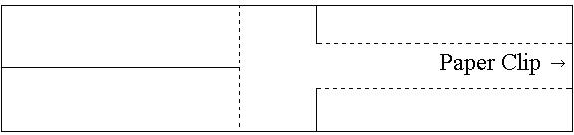
\includegraphics[width=0.45\textwidth]{./img/helicopter-1.png}
\caption{Paper helicopter template}
\label{fig:helicopter-1}
\end{center}
\end{figure}

\begin{figure}[h!]
\begin{center}
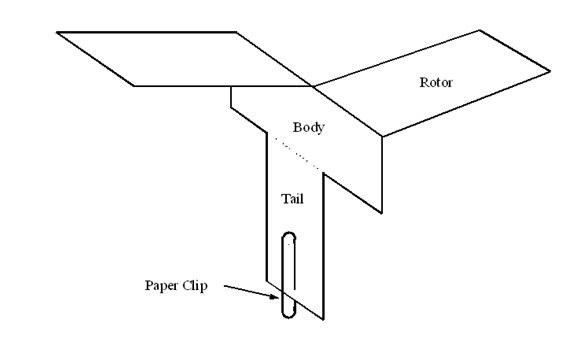
\includegraphics[width=0.6\textwidth]{./img/helicopter-2.png}
\caption{Paper helicopter construction}
\label{fig:helicopter-2}
\end{center}
\end{figure}